\documentclass{beamer}

\usepackage{color}
\usepackage[
%english
ngerman
]{babel}
\usepackage[ruled,linesnumbered]{algorithm2e}
\usepackage[T1]{fontenc}
\usepackage[%
%	latin1,
	utf8
]{inputenc}
\usepackage{ifthen}
\usepackage{rotating}
\usepackage{graphicx}
\usepackage{listings}
\lstset{basicstyle=\tiny,language=c,emphstyle=\col or{red},columns=fullflexible, keepspaces=true, keywordstyle=\tiny\color{blue}, showstringspace=true} 

\setbeamertemplate{navigation symbols}{}
%\setbeamertemplate{footline}[page number]
\setbeamertemplate{footline}[frame number]

\title{Einrichten eines Clusters zum Einspielen von Wikipedia-Traces}
\author{Praktikum Paralleles Rechnen (SS11)\\~\\Sebastian Menski}
%\institute{Institute of Computer Science\\University of Potsdam}
\institute{Institute für Informatik\\Universität Potsdam}
\date{19. Juli 2011}

\begin{document}

\frame{\thispagestyle{empty}\titlepage}
\frame{\thispagestyle{empty}\tableofcontents{}}

\newcommand{\mytitle}{}

\newcommand{\mysection}[1]{
\renewcommand{\mytitle}{#1}
\section{#1}
% \frame{\thispagestyle{empty}
% \begin{center}
% \textcolor{beamer@blendedblue}{\LARGE\mytitle}
% \end{center}
% }
}

\newcommand{\myframe}[2][\empty]{
\frame{\frametitle{\mytitle}
  \ifthenelse{\equal{#1}{\empty}}
    {#2}
    {\framesubtitle{#1}#2}
}
}

\newcommand{\mybreakframe}[2][\empty]{
\frame[allowframebreaks]{\frametitle{\mytitle}
  \ifthenelse{\equal{#1}{\empty}}
    {#2}
    {\framesubtitle{#1}#2}
}
}
\newcommand{\myfframe}[2][\empty]{
\frame[fragile]{\frametitle{\mytitle}
  \ifthenelse{\equal{#1}{\empty}}
    {#2}
    {\framesubtitle{#1}#2}
}
}


\mysection{Motivation}

\myframe{
  \begin{itemize}
  \item Doktorarbeit von Jörg Zinke
  \item Server Load Balancing Benchmark
  \item Realistisches Szenario bzw. Anwendung
  \item Einspielen von originalen Wikipedia-Traces
  \item Vorhanden\footnote{\url{http://www.wikibench.eu} \cite{wikibench}}:
    \begin{itemize}
    \item Wikipedia-Traces (18. September 2007 - 3. Januar 2008)
    \item englischer Wikipedia-Dump (3. Januar 2008)
    \end{itemize}
  \end{itemize}
}

\myframe[Leistungsanalyse: Messen, Modellieren und Simulation (WS10/11)]{
  \begin{itemize}
  \item Fabian Hahn \cite{fhahn}
  \item Perlbal Load Balancer mit httperf und den Wikipedia-Traces testen
  \item Erkenntnisse:
    \begin{itemize}
    \item Wikipedia-Dump enthält keine Bilder
    \item Einspielen des Dumps ist zeitaufwendig und instabil
    \item Es existiert ein Crawler um die Bilder nachzuladen
    \item Die Thumbnails werden dynamisch beim Aufrufen des Wikipedia-Artikels erzeugt
    \item Traces rufen Thumbnails direkt auf
    \item Serielles aufrufen aller Wikipedia-Artikel sehr zeitaufwendig  
    \end{itemize}
  \end{itemize}
}

\myframe[Aufgabestellung]{
  \begin{itemize}
  \item Aufsetzen mehrer Wikipedia-Instanzen auf dem IB-Cluster
  \item Erstellen einer parallelen Anwendung zum Aufrufen aller Wikipedia-Artikel vom Leibniz-Cluster aus
  \end{itemize}
}

\mysection{Erster Versuch}

\myframe[Ausgangsituation]{
  \begin{itemize}
  \item Wikipedia-Dump: 14GB (6.226.028 Wikipedia-Artikel; nur englische Wikipedia)
  \item Bilder (Stand 24.05.2011):
    \begin{itemize}
    \item 347GB
    \item 984.641 Dateien 
      \begin{description}
      \item[JPEG:] 72,34\%
      \item[PNG:] 18,06\%      
      \item[SVG:] 5,97\%
      \item[GIF:] 3,03\%
      \end{description}

    \end{itemize}
  \item Mediawiki 1.16.5
  \item IB-Cluster: 8 Nodes
  \item Leibniz-Cluster: 15 Nodes
  \end{itemize}
}

\myframe[IB-Cluster (Stand: 24.05.2011)]{
\begin{table}
  \centering
  \begin{tabular}{|c|ccc|}\hline
    Node & ib1-4 & ib5/ib6 & ib7/ib8 \\\hline
    CPU &  Intel Xenon  & Intel Pentium 4& 2x Intel Xenon \\
        & 2,66GHz  & 2,8GHz & 1,86GHz \\
    Cores &  1 & 1 & 2 \\
    RAM & 1GB & 4GB & 4GB \\\hline
  \end{tabular}
  \caption{IB-Cluster Nodes}
  \label{tab:ibold}
  \begin{itemize}
  \item CentOS 5.6
  \item Alle Nodes 33GB /
  \item ib6/ib7 1TB /data
  \end{itemize}
\end{table}
}

\myframe[Leibniz-Cluster] {
  \begin{table}
    \centering
    \begin{tabular}{|c|cc|}\hline
      Node & node001-010 & node011-015\\\hline
      CPU & 2x AMD Opteron 244 & Intel Xeon E5520 \\
          & 1,8GHz & 2,27GHz\\
      Cores & 2 & 4 \\
      RAM & 4GB & 6GB \\\hline
      
    \end{tabular}
    \caption{Leibniz Nodes}
    \label{tab:leibnizold}
  \end{table}
}

\myframe[Umsetzung (Stand: 24.05.2011)]{
  \begin{description}
  \item[ib1:] LVS Load Balancer mit least connections ohne Gewichte
  \item[ib2-4:] MySQL und Apache lokal (NFS ib6:/data)
  \item[ib5/ib8:] MySQL und Apache lokal (NFS ib7:/data)
  \item[ib6:] MySQL, Apache und /data lokal
  \item[ib7:] MySQL, Apache und /data lokal
  \item[leibniz:] Liste aller Wikipedia Artikel; Python Skript (Threading, Async, HTTP1.0/1.1)
  \end{description}
}

\myframe[Probleme]{
  \begin{itemize}
  \item Speicherplatz
    \begin{itemize}
    \item MySQL Datenbank mit eingespielten Wiki-Dump: ca. 25GB
    \item Speicher auf / verfügbar: ca. 29GB
    \item Bilder müssen in Datenbank eingelesen werden (Speicherung von Metadaten)
    \item Folge: MySQL Datenbank passt nicht mehr auf /
    \item Lösung: MySQL über Netzwerk aber bereits /data über NFS
    \end{itemize}
  \item Thumbnail Generierung:
    \begin{itemize}
    \item Nicht genau feststellbar ob Thumbnails erfolgreich generiert wurden
    \item ulimit Probleme (Lösung: Anpassung der Mediawiki Einstellungen)
    \item Imagemagick segmentation fault beim Umwandeln von SVG (Redhat Bug im Paket gnome-vfs2)
    \end{itemize}
  \item ib1-4 sehr alt und instabil
  \item Mediawiki alles andere als stabil und schnell
  \end{itemize}
}

\myframe[Fazit]{
  \begin{itemize}
  \item riesige Datenmengen
  \item Speicherplatz Mangel
  \item MySQL über Netzwerk und NFS verfälschen Messergebnisse
  \item Brauchen wir wirklich alle Bilder und Thumbnails?
  \end{itemize}
}

\mysection{Neue Aufgabenstellung}

\myframe{
  \begin{itemize}
  \item Gespräch: Frau Schnor, Jörg Zinke und Sebastian Menski (09.06.2011)
  \item Resultat:
    \begin{itemize}
    \item Jörg wählt 30 Minuten aus dem Trace aus
    \item Sebastian erstellt eine Skript, das die Wikipedia Instanz für genau diese 30 Minuten einrichtetA
    \item Filtern:
      \begin{itemize}
      \item http://en.wikipedia.org
      \item http://upload.wikimedia.org/wikipedia/commons/
      \item http://upload.wikimedia.org/wikipedia/en/
      \end{itemize}

    \end{itemize}
  \end{itemize}
}

\myframe[Trace Ausschnitt] {
  \begin{description}
  \item[tracefile:] wiki.1194899823.gz
  \item[start time:] Mon, 12 Nov 2007 18:31:30 +0000
  \item[end time:] Mon, 12 Nov 2007 19:31:35 +0000
  \item[duration:] 3604.986 sec
  \item[lines:] 17.518.902
  \item[requests:] 17.518.817
  \item[errors:] 85
  \end{description}

  Trace Zeile:\\
  \tiny{5396292369 1194892290.546 http://en.wikipedia.org/wiki/Travis\_Barker -}
}

\myframe[Trace Ausschnitt - Request pro Sekunde]{
  \begin{figure}
    \centering
    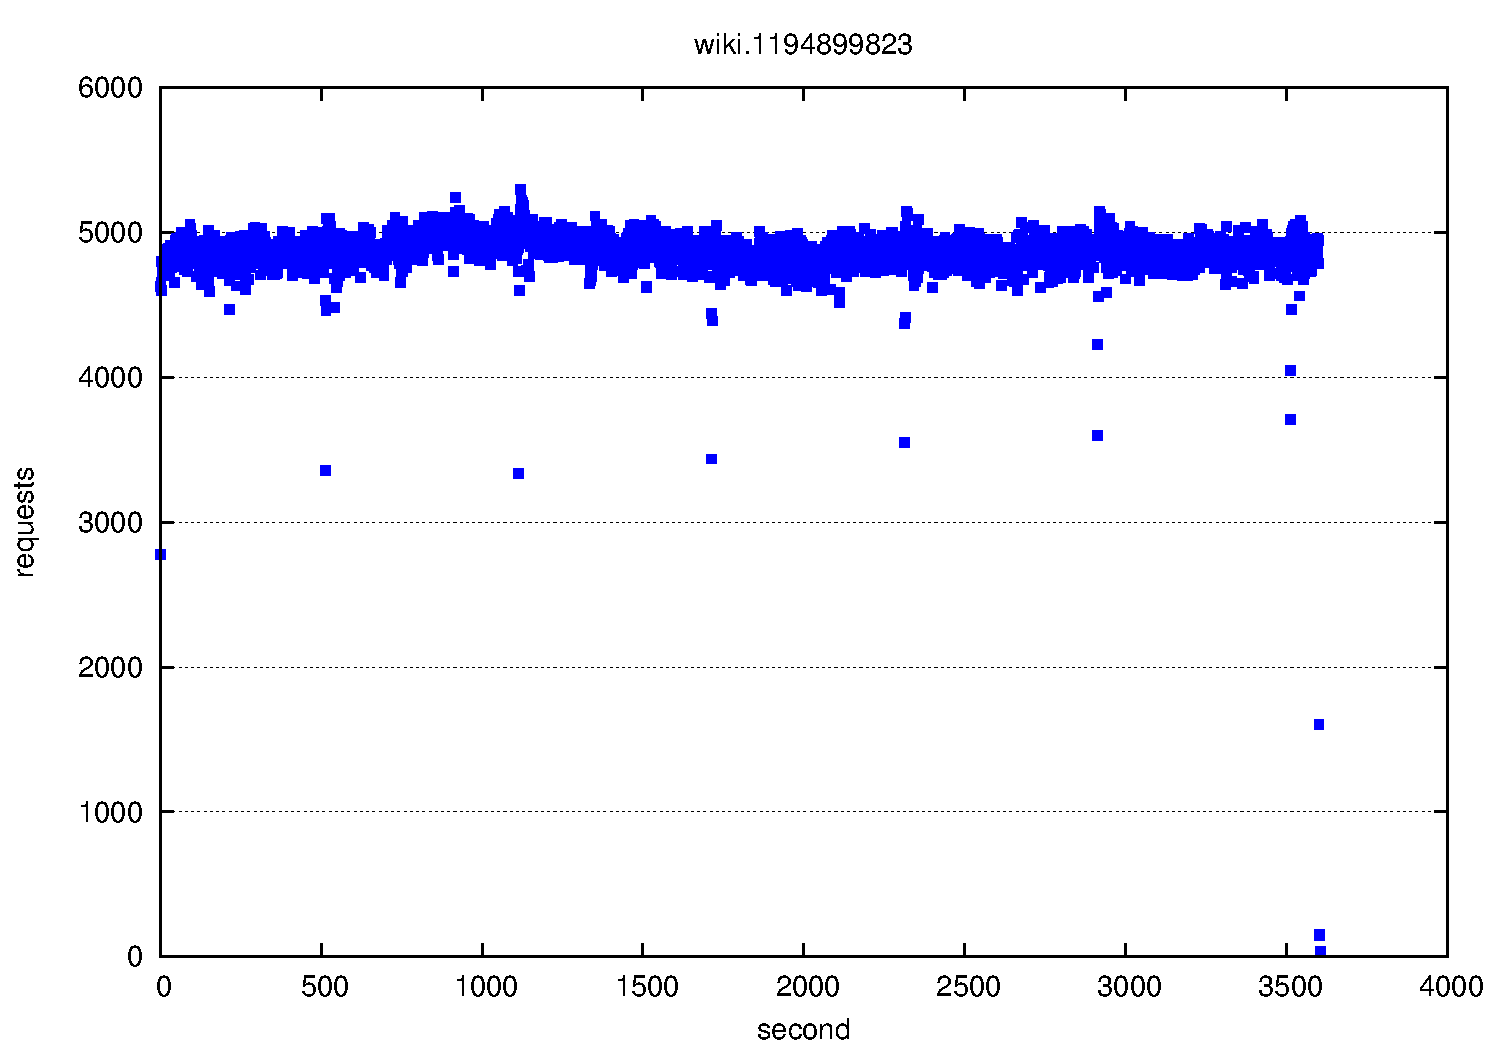
\includegraphics[width=\linewidth]{plot/trace}
  \end{figure}
}

\myframe[Trace Ausschnitt (gefiltert)] {
  \begin{description}
  \item[tracefile:] wiki.1194899823.1194892290-1194894090.gz
  \item[start time:] Mon, 12 Nov 2007 18:31:30 +0000
  \item[end time:] Mon, 12 Nov 2007 19:01:30 +0000
  \item[duration:] 1800.788 sec
  \item[lines:] 4.795.845
  \item[requests:] 4.795.845
  \item[errors:] 0
  \item[upload.wikimedia.org:]  3.196.418 (66,6\%)
  \item[en.wikipedia.org:]  1.599.427 (33,3\%)
  \end{description}
}

\myframe[Trace Ausschnitt (gefiltert) - Requests pro Sekunde] {
  \begin{figure}
    \centering
    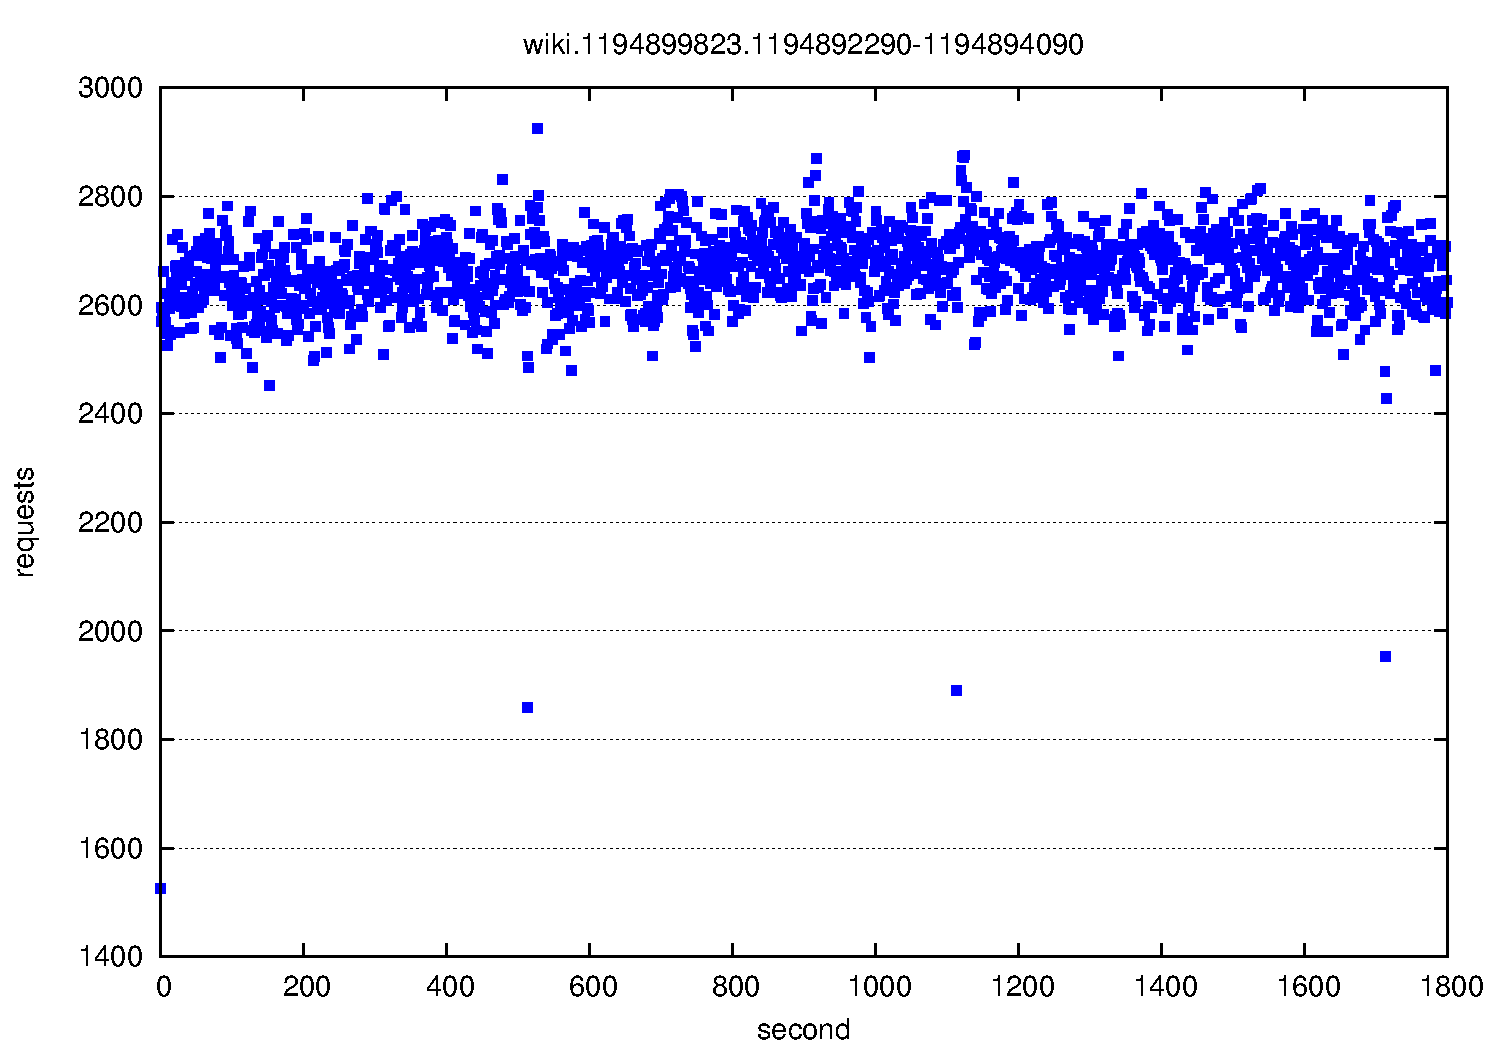
\includegraphics[width=\linewidth]{plot/trace-part}
  \end{figure}
}


\mysection{Zweiter Versuch}

\myframe[Idee]{
  \begin{enumerate}
  \item Filtern des Traces
  \item Download aller enthaltenen Bilder im gefilterten Trace
  \item Download aller enthaltenen Thumbnails im gefilterten Trace
  \item Importieren der Bilder in die Datenbank
  \item Bilder und Datenbank packen
  \item Bilder und Datenbank auf anderen Server installieren
  \end{enumerate}
}

\myframe[Grundlagen]{
  \begin{itemize}
  \item Python2.6 (für den Download)
  \item Python2.4 (für die Installation auf den Servern)
  \item ib5-8: besitzen 1TB /data für die Datenbank
  \item ib2-4: lokal Bilder; Datenbank über Netzwerk
  \item ib1: LVS Load Balancer
  \item Verluste:
    \begin{itemize}
    \item ib1/2/3: irreparabel defekt
    \item ib1-4 durch anderen Maschinen ersetzt
    \end{itemize}
  \end{itemize}
}

\myframe[IB-Cluster (Stand: 19.07.2011)]{
\begin{table}
  \centering
  \begin{tabular}{|c|ccc|}\hline
    Node & ib1-4 & ib5/ib6 & ib7/ib8 \\\hline
    CPU &  2x AMD Opteron 244  & Intel Pentium 4 & 2x Intel Xenon \\
        & 1,8GHz  & 2,8GHz & 1,86GHz \\
    Cores &  2 & 1 & 2 \\
    RAM & 4GB & 4GB & 4GB \\\hline
  \end{tabular}
  \caption{IB-Cluster Nodes}
  \label{tab:ibnew}
  \begin{itemize}
  \item CentOS 5.6
  \item ib1: 143GB /
  \item ib2: 69GB /
  \item ib3: 31GB /
  \item ib4: 69GB /
  \item ib5-8 33GB /; 1TB /data
  \end{itemize}
\end{table}
% 143GB ib1 69GB ib2 31GB ib3 69GB
}

\myframe[Python Skript I] {
  \begin{description}
  \item[Code:] \url{https://github.com/menski/ppr-s11}
  \item[Files:] 
    \begin{itemize}
    \item setup\_env.py (Hauptskript; benötigt Konfigurationsdatei)
    \item example.cfg (Beispiel Konfiguration)
    \item ppr/
      \begin{itemize}
      \item basic.py  (Basis Klassen)
      \item http.py   (Klassen für HTTP Requests und Download)
      \item server.py (Funktionen und Klassen zum ausführen von Befehlen)
      \item trace.py  (Klassen zum Analysieren und Filtern von Traces)
      \end{itemize}
    \end{itemize}
  \end{description}
}

\myframe[Python Skript II] {
  \begin{itemize}
  \item Fast jede Klasse ist ein Prozess
  \item Ablauf genau durch Konfigurationsdatei steuerbar
  \end{itemize}
}

\myframe[Konfiguration]{
 \begin{center}
 \textcolor{beamer@blendedblue}{\LARGE example.cfg}
 \end{center}
}

\mysection{Zusammenfassung}

\myframe{
  \begin{itemize}
  \item Bilder die in der aktuellen Wikipedia existieren werden heruntergeladen
  \item Das sind nicht alle Bilder
  \item Das Skript ermöglicht die volle Automatisierung der Einrichtung der Testumgebung
  \item Sofern Public-Key Authentifizierung möglich, komplett ohne Nutzerinteraktion
  \item Hohe Laufzeit, da große Datenmengen verarbeitet und transportiert werden müssen
  \item Zeitintensiv: Packen und übermitteln der Bilder und der Datenbank
  \end{itemize}
}

\mysection{Hinweise zum Einspielen}

\myframe{
  \begin{itemize}
  \item Der Response auf ein nicht existierendes Thumbnail ist '500 Internal Server Error' und nicht '404 Not Found'
  \end{itemize}
}


\appendix{}
\newcounter{finalframe}
\setcounter{finalframe}{\value{framenumber}}
\pagestyle{empty}
\renewcommand{\mytitle}{References}
\frame[allowframebreaks]{\frametitle{\mytitle}
 \bibliographystyle{plain}
 \bibliography{references}
}
\setcounter{framenumber}{\value{finalframe}}

\end{document}

%%% Local Variables: 
%%% mode: latex
%%% TeX-master: t
%%% End: 
